As we said in the first section, the product taken into analysis is a seasonal item. Using Google Trends, we were able to identify the region of maximum and minimum interest of the users regarding a Louis Vuitton scarf. In the graph below is clear that this product is searched primarily in the cold seasons and it is year after year more demanded by the customers. In the chart the x-axis represents a five year time period while the y-axis represents the popularity of the keywords "Louis Vuitton Scarf" searched on Google (100 is the moment of maximum interest while 0 is the minimum).
\makebox[\textwidth][c]{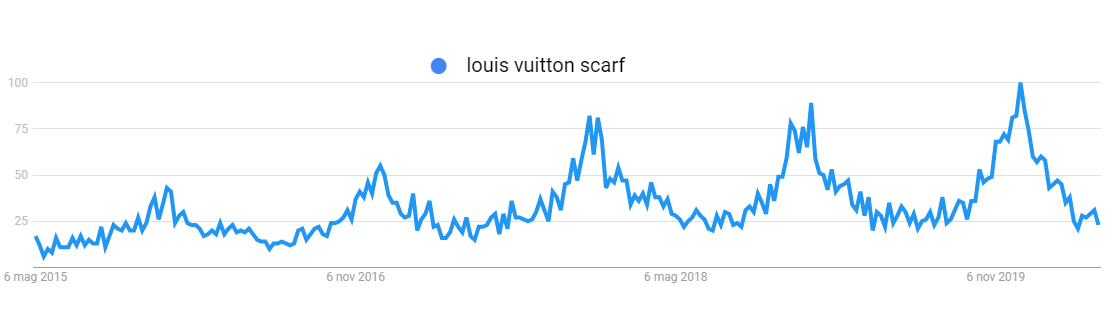
\includegraphics[width=1.2\textwidth]{sections/images/trend}}
Based on the diagram we decided to divide the year in four periods of time, each one underlining a different phase.\newline\\
\makebox[\textwidth][c]{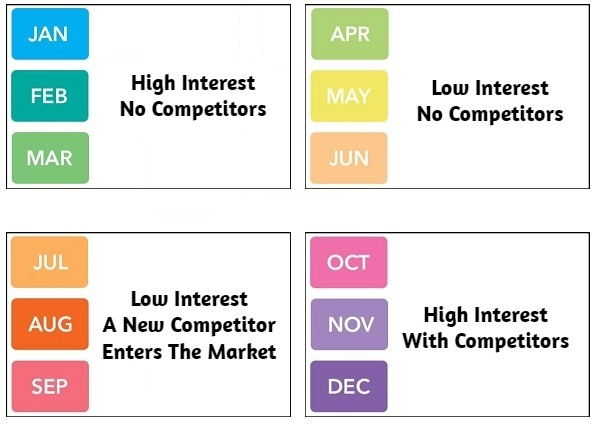
\includegraphics[width=0.8\textwidth]{sections/images/months}}
For each period of time a chart illustrating the probability distribution over the daily number of clicks for every value of budget allocated to that sub-campaign is provided.\newline
\makebox[\textwidth][c]{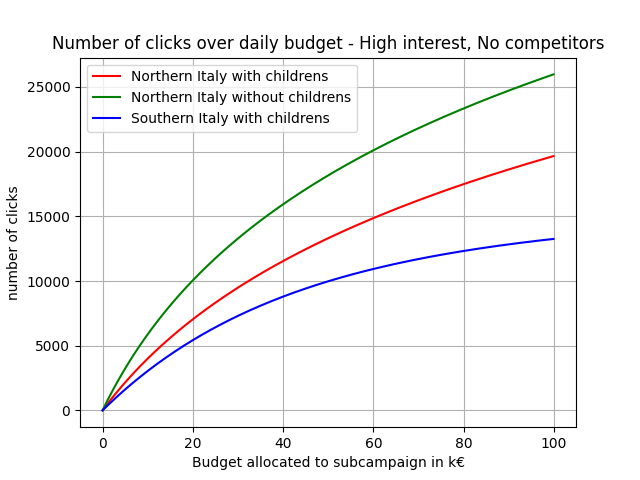
\includegraphics[width=0.85\textwidth]{../curves/real_curves/daily_clicks_10}} 
\makebox[\textwidth][c]{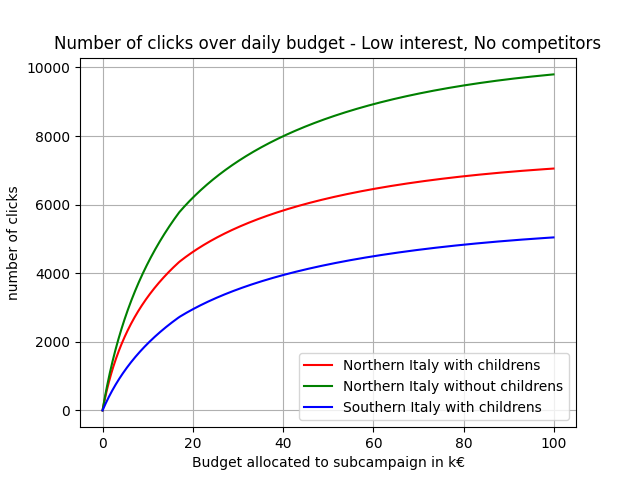
\includegraphics[width=0.85\textwidth]{../curves/real_curves/daily_clicks_00}} 
\makebox[\textwidth][c]{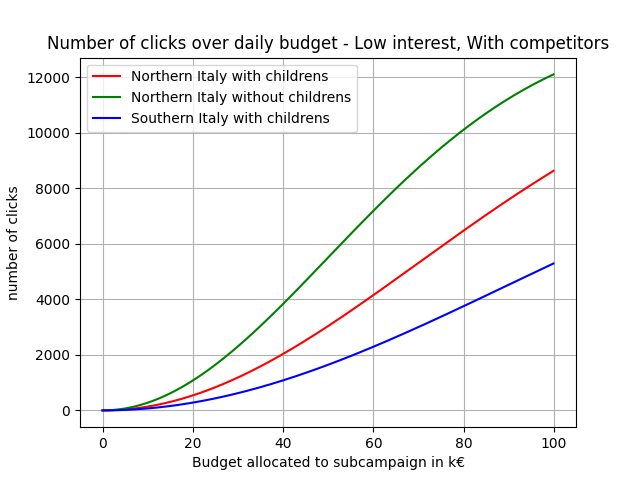
\includegraphics[width=0.85\textwidth]{../curves/real_curves/daily_clicks_01}} 
\newline\\\\
\makebox[\textwidth][c]{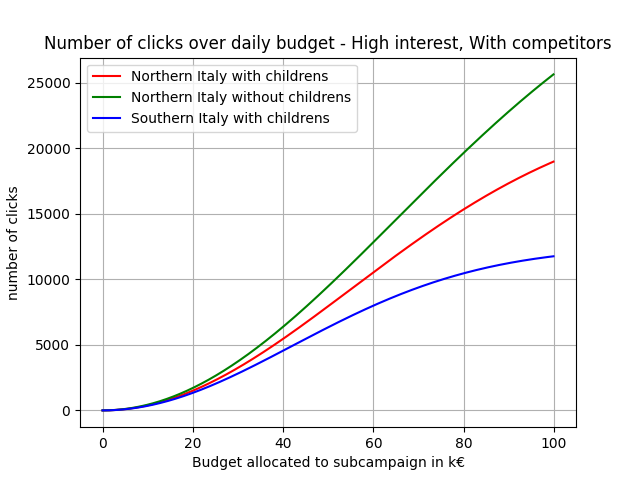
\includegraphics[width=0.85\textwidth]{../curves/real_curves/daily_clicks_11}} 